% 2006_sichuan_liberal_q9_fig1: sphere O with square pyramid P-ABCD on great circle
% schematic: outer circle solid, great-circle front solid / back dashed, pyramid edges dashed
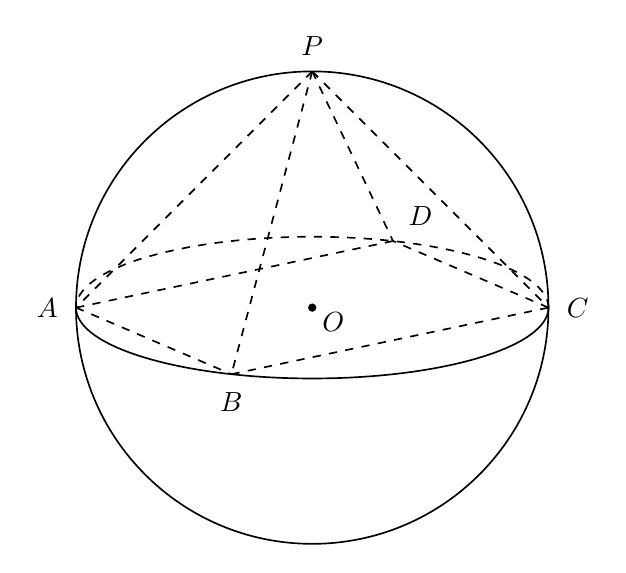
\begin{tikzpicture}[x=1cm,y=1cm,font=\normalsize,line width=.6pt]
\coordinate (O) at (0,0);
\coordinate (P) at (0.0000000000,3.0000000000);
\coordinate (A) at (-3.0000000000,0.0000000000);
\coordinate (B) at (-1.0260604300,-0.8457233587);
\coordinate (C) at (3.0000000000,0.0000000000);
\coordinate (D) at (1.0260604300,0.8457233587);
% sphere outline
\draw[solid] (O) circle (3);
% great circle as ellipse rx=2.8 ry=0.9: front (lower) solid, back (upper) dashed
\draw[solid,domain=180:360,samples=120] plot ({3*cos(\x)},{0.9*sin(\x)});
\draw[dashed,domain=0:180,samples=120] plot ({3*cos(\x)},{0.9*sin(\x)});
% pyramid lateral edges (all dashed in original)
\draw[dashed] (P) -- (A);
\draw[dashed] (P) -- (B);
\draw[dashed] (P) -- (C);
\draw[dashed] (P) -- (D);
% base perimeter
\draw[dashed] (A) -- (B);
\draw[dashed] (B) -- (C);
\draw[dashed] (C) -- (D);
\draw[dashed] (D) -- (A);
% base diagonals through great-circle diameter


% center dot
\fill (O) circle (1.5pt);
% labels kept clear of strokes
\node[above=2pt] at (P) {$P$};
\node[left=3pt] at (A) {$A$};
\node[below=3pt] at (B) {$B$};
\node[right=3pt] at (C) {$C$};
\node[above right=2pt] at (D) {$D$};
\node[below right=3pt,xshift=-3pt,yshift=5pt] at (O) {$O$};
\end{tikzpicture}
